\section{Early phase Yersinia Pestis infection}

Y. pestis differs from its evolutionary antecedent, Y. pseudotuberculosis in a few ways but one stands out. Y. pestis exhibits two phases in its pathogenesis of mammalian hosts. In the first, the bacteria are readily absorbed by host leukocytes via phagocytosis (white blood cells, mainly macrophages and neutrophils). Within macrophages especially, the bacteria replicates in relative shelter and secrecy from patrolling immune agents.\par
In the second phase, after a switching period, they prevent this absorption by a combination of resistance and neutralisation. This is probably to avoid the more aggressive neutrophils which arrive at the infected area after a period, with recruitment following pathogen detection. This work explores the mathematical implications of this switching in an attempt to quantify the significance of the strategy's evolutionary advantage.\par 


This shift in phase of the incident bacteria occurs in response to sensing the warmer ambient temperature of a mammalian host. At a cooler temperature inside a flee, the bacteria remains in its first phase. Then after the flea bites its host, injected bacteria will after some delay shift behaviour to the second phase. The key difference acquired is resistance to phagocytosis. At the outset of invasion, colony forming units will be absorbed (phagocytosed) by host macrophages. With evolved resistance to their toxins, Y. pestis bacteria use this intracellular refuge as a temporary home to replicate and bolster numbers against challenges to come. The first mounted attack of the innate immune system is neutrophils. Summoned by various cytokines, they arrive on the scene in numbers, passing through the walls of blood vessels to the extracellular matrix in which the infection is beginning to take hold. After some time, an infected macrophage will rupture and its resident bacterial population will disperse into the extracellular matrix. Those Y. pestis bacteria which have undergone the transition to the second phase are characterised by being resistant to further phagocytosis.  Figure \ref{fig:two_columns_six_image} illustrates the dynamics. 


\begin{figure}[h!]
    \centering
    % First row of two images
    \begin{subfigure}{0.48\textwidth}
        \centering
        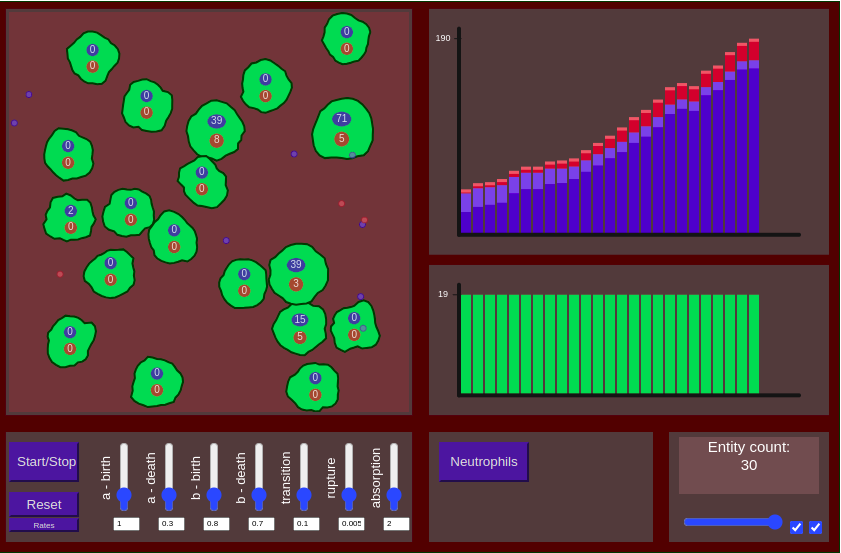
\includegraphics[width=\textwidth]{figures/fig_yp_schematic/web1}
    \end{subfigure}
    \hspace{\fill}
    \begin{subfigure}{0.48\textwidth}
        \centering
        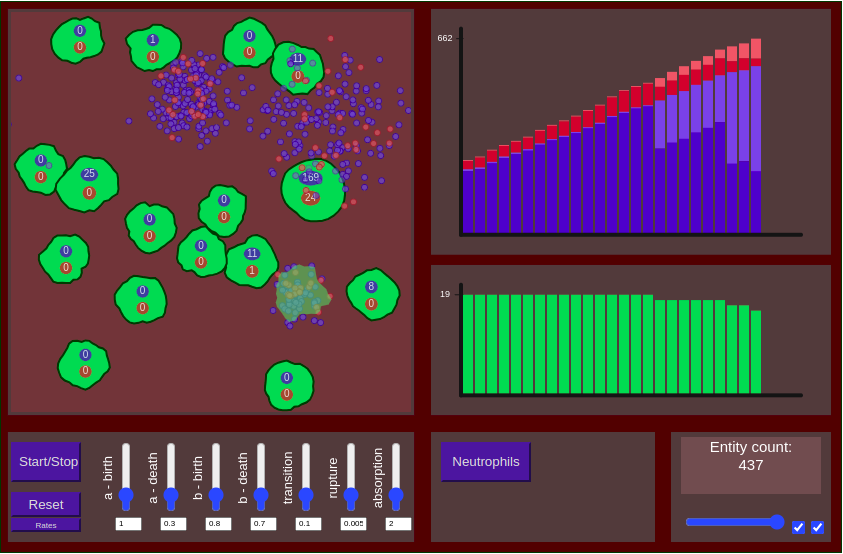
\includegraphics[width=\textwidth]{figures/fig_yp_schematic/web2}
    \end{subfigure}

\caption*{Bacterial replication takes place within macrophage.  Some phase transitions occur.}
    \vspace{0.5em} % Small vertical space between rows

    % Second row of two images
    \begin{subfigure}{0.48\textwidth}
        \centering
        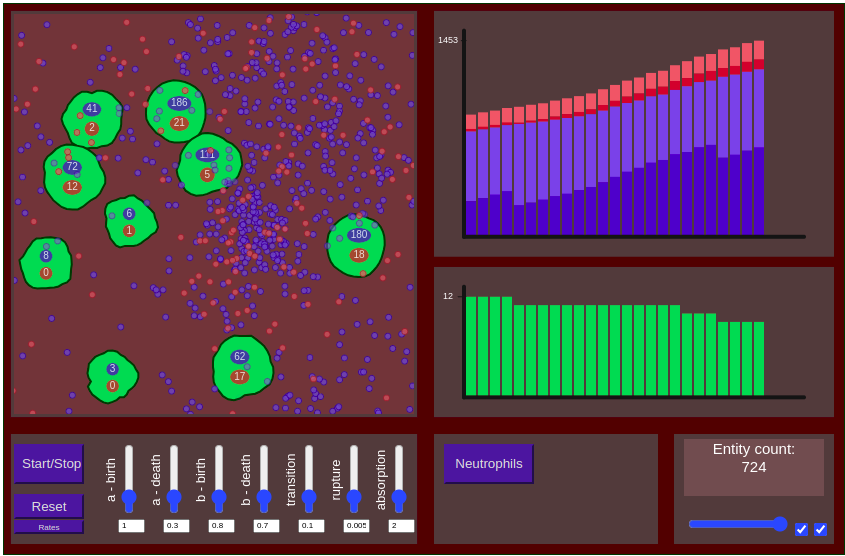
\includegraphics[width=\textwidth]{figures/fig_yp_schematic/web3}
    \end{subfigure}
    \hspace{\fill}
    \begin{subfigure}{0.48\textwidth}
        \centering
        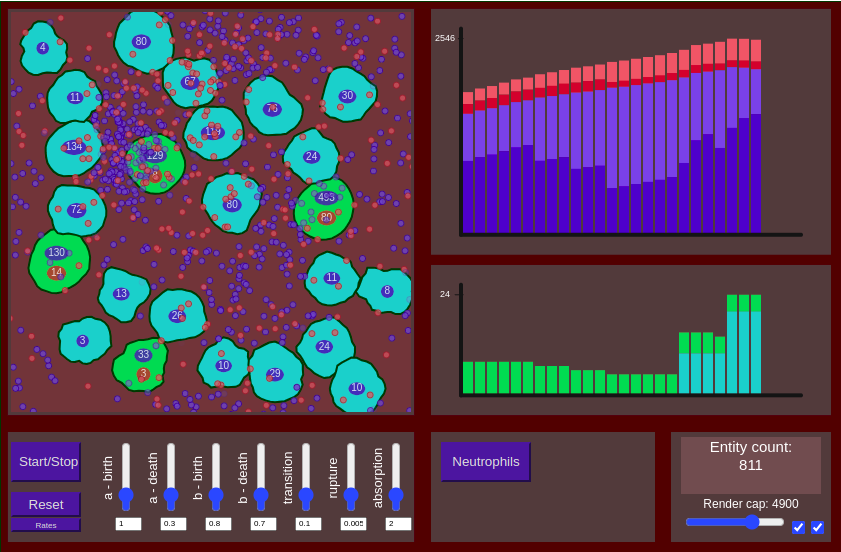
\includegraphics[width=\textwidth]{figures/fig_yp_schematic/web4}
    \end{subfigure}

\caption*{Macrophage bursting,  more transitions to the second phase (red particles).  Neutrophils arrive.}
    \vspace{0.5em} % Small vertical space between rows

    % Third row of two images
    \begin{subfigure}{0.48\textwidth}
        \centering
        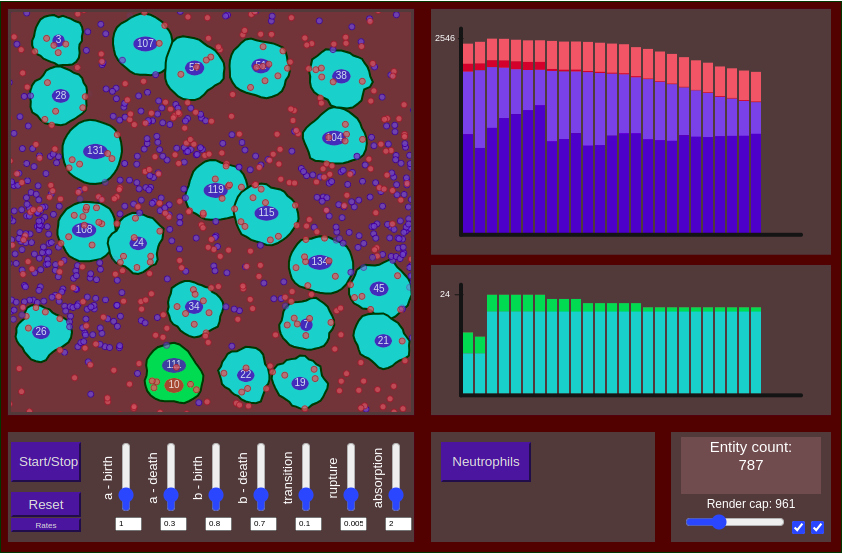
\includegraphics[width=\textwidth]{figures/fig_yp_schematic/web5}
    \end{subfigure}
    \hspace{\fill}
    \begin{subfigure}{0.48\textwidth}
        \centering
        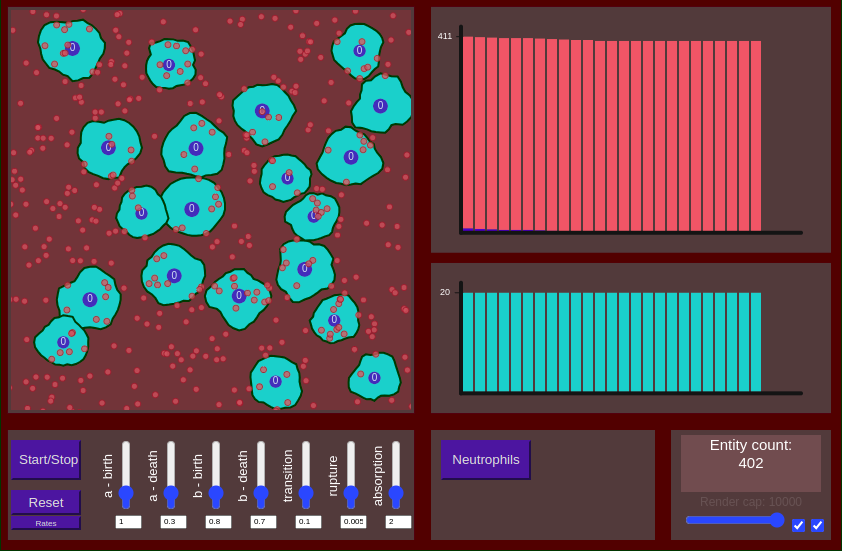
\includegraphics[width=\textwidth]{figures/fig_yp_schematic/web6}
    \end{subfigure}

    % Single caption for all images
\caption*{Neutrophils phagocytose and eliminate remaining phase one leaving Y. pestis as a primarily extracellular infection.}
    \caption{A schematic representation.}
    \label{fig:two_columns_six_image}
\end{figure}
